\newpage

\section{Análise dos Resultados}

Os resultados do MSL mostram que o Android foi a principal plataforma dos \emph{apps} desenvolvidos pelos estudos.
Sendo 9 aplicativos desenvolvidos somente para Android, 4 multiplataforma (Android e iOS) e 2
apenas para iOS, como mostra a \autoref{tab-tec-pla-des-1}.

\begin{table}[htb]
    \begin{center}
        \caption{Tecnologias utilizadas no desenvolvimento e plataforma alvo das aplicações.}
        \label{tab-tec-pla-des-1}
        \begin{tabular}{p{1.0cm}|p{8.0cm}|p{3.0cm}}
            %\hline
            \textbf{Artigo} & \textbf{Tecnologias}                                             & \textbf{Plataforma}  \\
            \hline
            AM1             & \emph{Cordova Framework}                                         & \emph{Android e iOS} \\
            \hline
            AM2             & \emph{MD², Xtend, Java, Eclipse}                                 & \emph{Android e iOS} \\
            \hline
            AM3             & \emph{Unity 3D engine, Java}                                     & Android       \\
            \hline
            AM4             & \emph{Android Studio 2.0}                                        & Android       \\
            \hline
            AM5             & Não informado                                                    & Android       \\
            \hline
            AM6             & \emph{Java, Android Studio, Accessibility Scanner App, Test Lab} & Android       \\
            \hline
            AM7             & Não informado                                                    & Android       \\
            \hline
            AM8             & Não informado                                                    & iOS           \\
            \hline
            AM9             & Não informado                                                    & iOS           \\
            \hline
            AM10            & \emph{React Native}                                              & \emph{Android e iOS} \\
            \hline
            AM11            & Não informado                                                    & Android       \\
            \hline
            AM12            & \emph{Java, Android Studio, API Airy}                            & Android       \\
            \hline
            AM13            & Não informado                                                    & Android       \\
            \hline
            AM14            & Não informado                                                    & Android       \\
            \hline
            AM15            & \emph{React Native}                                              & \emph{Android e iOS} \\
            % \hline
        \end{tabular}
        \legend{Fonte: Autor.}
    \end{center}
\end{table}

Embora todos os estudos tenham mencionado a plataforma para qual o \emph{app} foi desenvolvido,
como pode ser observado na \autoref{tab-tec-pla-des-1}, boa parte deles, 7 no total, não mencionam as tecnologias utilizadas.
Com isso, \emph{Java} destacou-se como a principal linguagem, utilizada em pelo menos 4 estudos, para o desenvolvimento das soluções.
Enquanto o \emph{React Native} apareceu como principal o \emph{framework} para desenvolvimento multiplataforma com duas aplicações.

\newpage

Quanto às técnicas relacionadas à acessibilidade utilizadas no desenvolvimento das soluções apresentadas nos artigos, são listadas
na \autoref{tab-tec-uti-des-1} as principais identificadas no MSL\@.
Nessa tabela foi atribuído um código de referência para cada técnica listada.

\begin{table}[htb]
    \begin{center}
        \caption{Técnicas utilizadas no desenvolvimento das soluções de acessibilidade do MSL.}
        \label{tab-tec-uti-des-1}
        \begin{tabular}{p{1.2cm}|p{9.2cm}|p{4.1cm}}
            %\hline
            \textbf{Código} & \textbf{Técnicas}                                                                                  & \textbf{Artigos}                                                     \\
            \hline
            TAM1            & Contraste de cor para garantir diferentes níveis de acessibilidade                                 & AM1, AM9, AM10, AM12, AM13                                           \\
            \hline
            TAM2            & Descrição textual dos elementos visuais                                                            & AM1, AM2, AM3, AM5, AM6, AM7, AM8, AM9, AM10, AM11, AM12, AM13, AM15 \\
            \hline
            TAM3            & Escala SUS para avaliação da usabilidade da aplicação                                              & AM4, AM5, AM7                                                        \\
            \hline
            TAM4            & Elementos chave de interação sempre posicionados na mesma parte da tela, em locais de fácil acesso & AM10, AM15                                                           \\
            \hline
            TAM5            & \emph{Feedback} por vibração                                                                       & AM3, AM14                                                            \\
            \hline
            TAM6            & \emph{Feedback} por voz por meio de TTS                                                            & AM3, AM5, AM6, AM7, AM9, AM11, AM12, AM13, AM14                      \\
            \hline
            TAM7            & Interação alternativa fazendo uso de de gestos                                                     & AM1, AM7, AM10, AM12, AM15                                           \\
            \hline
            TAM8            & Personalização de pontos da \emph{interface} que afetam a acessibilidade                           & AM2, AM6, AM8, AM9, AM12                                             \\
            \hline
            TAM9            & Possibilidade de revisar as mensagens escritas por meio de TTS                                     & AM7                                                                  \\
            \hline
            TAM10           & Reconhecimento de voz                                                                              & AM4, AM6, AM7, AM9, AM12                                             \\
            \hline
            TAM11           & Tamanho da fonte das letras ampliado ou personalizável                                             & AM6, AM8, A12                                                        \\
            \hline
            TAM12           & Tamanho dos botões e espaçamentos adequados à PDV                                                  & AM9                                                                  \\
            \hline
            TAM13           & Tamanho dos ícones e componentes adaptáveis de acordo com tamanho da tela                          & AM10                                                                 \\
            \hline
            TAM14           & Todos os elementos visíveis na tela sem necessidade de rolagem                                     & AM10                                                                 \\
            \hline
            TAM15           & Utilização de efeitos sonoros para contextualizar o usuário                                        & AM3, AM6, AM13                                                       \\
            % \hline
        \end{tabular}
        \legend{Fonte: Autor.}
    \end{center}
\end{table}

A coluna ``Artigos'' na \autoref{tab-tec-uti-des-1} indica em quais artigos (representados por código) cada técnica foi identificada.
Como as descrições das técnicas identificadas variaram de acordo com os artigos, elas foram representadas nessa tabela
com uma descrição genérica, possibilitando a identificação dos artigos que utilizaram as mesmas técnicas.

\newpage

Os problemas mapeados pelos estudos relacionados, apresentados na \autoref{tab-pro-est-rel-1}, foram generalizados e divididos de acordo com as categorias
da \autoref{tab-cat-dir-acc-5}, definidas por \citeonline{Quispe2020}. O autor utilizou o eMAG como base,
alterando apenas a primeira categoria chamada ``Marcação'', que refere-se à linguagens de marcação da \emph{web},
para ``Estrutura'', ainda mantendo o mesmo sentido de organização e estrutura dos elementos de \emph{interface}.

\begin{table}[htb]
    \begin{center}
        \ABNTEXfontereduzida
        \caption{Principais problemas identificados pelos estudos relacionados.}
        \label{tab-pro-est-rel-1}
        \begin{tabular}{p{1.1cm}|p{4.0cm}|p{2.4cm}|p{6.7cm}}
            %\hline
            \textbf{Código} & \textbf{Problema}                                              & \textbf{Categoria}           & \textbf{Códigos de referência dos problemas}                                                                                                           \\
            \hline
            CPER1           & \emph{Feedback} auditivo não é suficiente para a interação     & Conteúdo / Informação        & AR4P14, AR4P15, AR4P47, AR4P50, AR4P52, AM1P3                                                                                                          \\
            \hline
            CPER2           & Apresentação dos conteúdos                                     & Apresentação / \emph{Design} & AM1P1, AM1P5, AM1P7, AM1P10, AR1P5, AR1P6, AR1P7, AR1P8, AR1P9, AR1P11, AR1P14                                                                         \\
            \hline
            CPER3           & Descrição textual inadequada/inexistente dos elementos de tela & Conteúdo / Informação        & AR1P8, AM1P4, AR1P1, AR1P2, AR1P4, AR1P7, AR1P10, AR4P11, AR1P14, AR4P49, AR4P59, AM1P4                                                                \\
            \hline
            CPER4           & Dificuldades ao navegar pela aplicação                         & Estrutura                    & AM1P1, AM1P5, AM1P6, AM1P8, AM1P9, AR1P5, AR1P8, AR4P46                                                                                                \\
            \hline
            CPER5           & Dificuldades com a utilização do teclado virtual padrão        & Formulários                  & AR4P16, AR4P17, AR4P19, AR4P20, AR4P21, AR4P22, AR4P23, AR4P24, AR4P25, AR4P26                                                                         \\
            \hline
            CPER6           & Dificuldades relacionadas a botões virtuais                    & Apresentação / \emph{Design} & AR4P1, AR1P2, AR4P2, AR1P10                                                                                                                            \\
            \hline
            CPER7           & Dificuldades na utilização de gestos                           & Comportamento                & AR4P27, AR4P28, AR4P29, AR4P30, AR4P31, AR4P32, AR4P33, AR4P34, AR4P35, AR4P36, AR4P37, AR4P38, AR4P39, AR4P40, AR4P41, AR4P42, AR4P43, AR4P44, AR4P45 \\
            \hline
            CPER8           & Dificuldades com leitor de tela                                & Comportamento                & AM1P7, AM1P2, AR4P46, AR4P47, AR4P48, AR4P50, AR4P51, AR4P53, AR4P54, AR4P55, AR4P56, AR4P57, AR4P58, AM1P3                                            \\
            \hline
            CPER9           & Funcionalidades confusas ou não claras                         & Estrutura                    & AR1P3, AR1P4, AR1P6, AR1P9, AR1P10, AR1P11, AM1P6, AM1P8                                                                                               \\
            \hline
            CPER10          & Obstáculos relacionados ao reconhecimento de voz               & Comportamento                & AR4P3, AR4P4, AR4P5, AR4P6, AR4P7, AR4P8, AR4P9, AR4P10                                                                                                \\
            % \hline
        \end{tabular}
        \legend{Fonte: Autor.}
    \end{center}
\end{table}
A \autoref{tab-tec-pro-1} relaciona os códigos de referência dos problemas listados na
\autoref{tab-pro-est-rel-1} com os códigos das diretrizes definidas pelos estudos relacionados e das principais
técnicas identificadas nos artigos do MSL, reunidas na \autoref{tab-tec-uti-des-1}.

\begin{table}[htb]
    \begin{center}
        \caption{Diretrizes e técnicas relacionadas à cada tipo de problema.}
        \label{tab-tec-pro-1}
        \begin{tabular}{p{2.0cm}|p{12.5cm}}
            %\hline
            \textbf{Código do problema} & \textbf{Diretrizes/Técnicas}                                                                                                  \\
            \hline
            CPER1                       & AR3D8, AR3D9, AR3D11, AR5R10, AR6D22, AR6D24, TAM5, TAM11, TAM13, TAM14                                                       \\
            \hline
            CPER2                       & AR3D1, AR3D2, AR3D5, AR3D8, AR3D9, AR3D11, AR5R6, AR5R8, AR5R10, AR6D3, AR6D4, AR6D10, AR6D14, AR6D24, TAM1, TAM8, TAM11      \\
            \hline
            CPER3                       & AR5R2, AR5R9, AR6D5, AR6D7, AR6D12, AR6D13, AR6D14, AR6D16, AR6D17, AR6D19, AR6D20, AR6D21, AR6D23, AR6D27, TAM2, TAM14       \\
            \hline
            CPER4                       & AR3D3, AR3D4, AR3D5, AR3D7, AR3D9, AR5R4, AR5R5, AR6D1, AR6D2, AR6D3, AR6D5, AR6D8, AR6D15, AR6D32, TAM4                      \\
            \hline
            CPER5                       & AR3D6, AR5R1, TAM9, TAM10                                                                                                     \\
            \hline
            CPER6                       & AR3D11, AR6D30, TAM12, TAM13                                                                                                  \\
            \hline
            CPER7                       & AR3D6, AR3D10, TAM6, TAM7, TAM9                                                                                               \\
            \hline
            CPER8                       & AR5R1, AR5R2, AR5R3, AR5R4, AR5R6, AR5R8, AR5R9, AR6D1, AR6D2, AR6D3, AR6D12, AR6D13, AR6D14, AR6D17, TAM2, TAM4, TAM6, TAM14 \\
            \hline
            CPER9                       & AR3D4, AR3D5, AR3D7, AR5R9, AR6D1, AR6D2, AR6D3, AR6D4, AR6D16, TAM4                                                          \\
            \hline
            CPER10                      & AR5R1, TAM10                                                                                                                  \\
            % \hline
        \end{tabular}
        \legend{Fonte: Autor.}
    \end{center}
\end{table}

\newpage

Como pode ser observado na \autoref{tab-tec-pro-1}, todos os tipos de problemas listados possuem alguma
técnica da \autoref{tab-tec-uti-des-1}, das técnicas identificadas no MSL, relacionada.

\subsection{CPER1: \emph{Feedback} auditivo não é suficiente para a interação}

Embora o retorno auditivo tenha sido o principal recurso utilizado para acessibilidade de PDV, como pode
ser visto na \autoref{tab-tec-uti-des-1}, existem várias limitações quanto à essa solução, mesmo considerando
que todos os elementos de tela tenham as descrições adequadas para narração pelos leitores de
telas.

Tais limitações referem-se a: entendimento da orientação e organização da \emph{interface}, utilização
em ambientes ruidosos, falta privacidade e pronúncia das palavras \cite{Damaceno2016}.
Com isso, faz-se necessário o suporte à outras formas de retorno acessível para o usuário, mediante a solução de outros problemas
listados, em destaque o CPER2 relacionado à \emph{interface}.

\subsection{CPER2: Apresentação dos conteúdos}

Problemas como a falta de consistência no \emph{layout}, a má organização dos conteúdos das telas e
funcionalidades e sequências de interação confusas podem levar a um não entendimento
da sequência de leitura e gerar sobrecarga de informações para o usuário \cite{Shera2021285, Christoph2020}.

Diante desses problemas, técnicas como posicionar os elementos chave de interação sempre na mesma posição,
adaptar o tamanho dos componentes de acordo com o tamanho da tela e evitar colocar muito conteúdo na tela para evitar
a rolagem podem ser bastante úteis \cite{Mascetti2019,Ducci2018}. Suporte ao alto contraste,
esquemas alternativos de cores, ampliação da tela e fontes maiores e mais legíveis também podem ajudar nesse sentido
\cite{Kim20191103,Oliveira2019}.

\subsection{CPER3 e CPER8: Problemas relacionados às descrições dos elementos e leitores de tela}

Problemas relacionados a leitores de tela e descrições textuais dos elementos apareceram com alta frequência na \autoref{tab-pro-est-rel-1},
justificando a técnica TAM2, da \autoref{tab-tec-uti-des-1}, ter sido a mais utilizada nos estudos e a mais discutida por
desenvolvedores no Stack Overflow \cite{Vendome201941}.

A técnica TAM2 refere-se à descrição textual dos elementos de tela e sua utilização foi mencionada explicitamente em 13 dos
15 artigos selecionados no MSL\@. Além dela, a técnica TAM6 que fornece o \emph{feedback} auditivo nativamente nas aplicações,
por meio TTS também foi uma das técnicas mais utilizadas, como pôde ser visto na \autoref{tab-tec-uti-des-1}. Assim, mostrando-se
uma possível alternativa para o problema com \emph{crash} do leitor de telas citado por \citeonline{Shera2021285}.

\subsection{CPER4: Dificuldades ao navegar pela aplicação}

Diversos problemas de navegação associados também ao CPER2, de apresentação dos conteúdos, foram encontrados, particularmente:
o não entendimento do fluxo de tarefas e a falta de consistência na organização dos conteúdos/\emph{layout}
\cite{Shera2021285,Christoph2020,Quispe2020}. Outro problema dá-se pela forma de navegação entre os elementos dos leitores de tela,
que é linear, demorando para ter-se uma noção geral da \emph{interface} \cite{Damaceno2016}.

Portanto, a preocupação com uma navegação intuitiva, posicionando elementos chave como caixas de pesquisa sempre no mesmo
local mostra-se fundamental para resolver alguns desses problemas \cite{Kim20191103,Mascetti2019,Ducci2018}.
A utilização de estratégias para o uso de leitores de tela, como atalhos atalhos para facilitar a navegação do usuário com DV
pela aplicação, principalmente um que possibilite que o usuário retorne a um lugar conhecido, como a tela inicial do \emph{app},
foi definida como essencial por \citeonline{Siebra2018172}, a partir de uma análise realizada com envolvimento de 5 PDV\@.

\subsection{CPER5: Dificuldades com a utilização do teclado virtual padrão}

Vários problemas relacionados à utilização do teclado virtual padrão foram identificados, como pode ser visto na
\autoref{tab-pro-est-rel-1}. Tornando ainda mais evidente a necessidade de possibilitar várias alternativas de interação
com as aplicações para usuários com DV\@, tanto de entrada de dados quanto de saída.

Algumas soluções como a possibilidade de \emph{feedback} auditivo dos caracteres que estão sendo digitados e
a de revisão do conteúdo escrito ao finalizar a digitação foram identificadas e validadas \cite{Siebra2016, Duarte2017}.
Além disso, o reconhecimento de voz, definido como diretriz por \citeonline{Kim20191103}, também foi
utilizado como alternativa ao uso de teclados virtuais por um terço dos estudos do MSL\@, como pode ser visto na \autoref{tab-tec-uti-des-1}.

\subsection{CPER6: Dificuldades relacionadas a botões virtuais}

No conjunto de problemas relacionados a botões levantado por \citeonline{Christoph2020}, são mencionados a falta de informações
e as funcionalidades confusas dos mesmos, porém, esses problemas estão associados ao CPER3, de descrições textuais
inadequadas/inexistentes das quais foram mencionadas outras soluções. Outros problemas com relação a esses botões são:
a grande proximidade entre eles e a menor sensibilidade tátil, em comparação com os botões físicos \cite{Damaceno2016}.

O uso de fontes legíveis com tamanho ampliado ou personalizável e o tamanho e espaçamento adequado para os botões virtuais
são essenciais, visto que podem dificultar a visualização para PDV parcial quando não estão utilizando leitores
de tela \cite{Heesook2017,Kim20191103}.

\subsection{CPER7: Dificuldades na utilização de gestos}

Como pôde-se visualizar na \autoref{tab-pro-est-rel-1}, problemas relacionados a gestos foram os mais frequentes, com a maioria dos usuários
que participaram do estudo de \citeonline{Oliveira2019} relatando ter enfrentado dificuldades, deixando algum comentário negativo a respeito.
Outro motivo para a dificuldade está na diferença entre os gestos das aplicações desenvolvidas e os habituais de cada plataforma \cite{Leporini2017}.

Contudo, resultados de outros estudos indicam que a utilização de gestos simples gerou \emph{feedbacks} positivos \cite{Duarte2017,Ducci2018}.

\subsection{CPER9: Funcionalidades confusas ou não claras}

Funcionalidades com apresentações não claras ou confusas, tanto pela descrição textual audível quanto pela visual, acabam
causando confusão nos usuários, os fazendo pensar que uma funcionalidade faz uma coisa quando na verdade faz outra \cite{Christoph2020}.

Esses problemas ressaltam ainda mais a importância de fornecer descrições textuais audíveis claras dos elementos de tela
e funcionalidades da aplicação, como é apontado no tópico específico do CPER3. Ao mesmo tempo, reforça também a importância
da apresentação visual dos conteúdos mencionada no tópico do CPER2.

\subsection{CPER10: Obstáculos relacionados ao reconhecimento de voz}

Diversas limitações com relação ao reconhecimento de voz foram levantadas por \citeonline{Damaceno2016}, algumas delas
são as mesmas citadas no tópico CPER1, sobre o \emph{feedback} auditivo não ser suficiente, por questões de privacidade,
ruídos de ambientes e pronúncia das palavras. Da mesma forma que o CPER1, faz-se necessário oferecer outros métodos
de entrada alternativos para os usuários, como resolver os problemas do tópico CPER5, associados a teclados virtuais.

Os outros problemas citados pelo autor, no mesmo estudo, foram o de apenas um comando ser reconhecido por vez, a necessidade
de mentalizar as instruções por voz, aumentando a carga de memória dos usuários, e o uso desses comandos ser computacionalmente
custoso. Para esses problemas não foram identificadas soluções nos estudos do MSL ou nos estudos relacionados.

\section{Respostas das Questões do Protocolo}

Nesta seção são respondidas as questões definidas no Protocolo de MSL, apresentado no início deste capítulo, levando em consideração a análise dos resultados da seção anterior.
Assim, seguem:

\begin{enumerate}
      \item Quais são as principais soluções de acessibilidade para PDV utilizadas
            no desenvolvimento de aplicações móveis?
            \begin{enumerate}
                  \item Foi observado o cumprimento de diretrizes de acessibilidade para aplicações móveis propostas por entidades
                        como Google\footnote{\url{https://developer.android.com/guide/topics/ui/accessibility/apps}},
                        SIDI\footnote{\url{https://www.sidi.org.br/guiadeacessibilidade}} e
                        BBC\footnote{\url{https://www.bbc.co.uk/accessibility/forproducts/guides/mobile}}; não foi identificado, porém, o uso das diretrizes da
                        Apple\footnote{\url{https://developer.apple.com/design/human-interface-guidelines/accessibility/overview/introduction/}};
                  \item Realização de estudos visando identificar problemas enfrentados por usuários com DV no uso de aplicativos móveis e definir diretrizes para solucionar cada problema;
                  \item Utilização de diretrizes de acessibilidade da W3C\footnote{\url{https://www.w3.org/TR/mobile-bp/summary}} adaptadas da \emph{web} para o contexto de aplicações móveis;
                  \item Utilização de ferramentas para realização de testes de acessibilidade automatizados.
            \end{enumerate}
      \item Quais são as tecnologias utilizadas no desenvolvimento dessas soluções?
            \begin{enumerate}
                  \item A linguagem Java no desenvolvimento de aplicações Android;
                  \item Os \emph{frameworks} React Native, Cordova e MD² no desenvolvimento multiplataforma;
                  \item As IDEs Android Studio e Eclipse;
                  \item Unity 3D no desenvolvimento de jogos para Android;
                  \item As ferramentas Accessibility Scanner App, MATE e Test Lab para realização de testes de acessibilidade automatizados.
            \end{enumerate}
      \item Para quais plataformas as soluções foram propostas?
            \begin{enumerate}
                  \item 9 apenas para Android;
                  \item 2 apenas para iOS\@;
                  \item 4 multiplataforma, para Android e iOS\@.
            \end{enumerate}
      \item Quem são os públicos alvos dessas soluções? \\
            As soluções visaram atender diversas necessidades de PDV\@.
            Assim, foram criadas aplicações para diferentes públicos com DV,
            como crianças e estudantes, e com diversos tópicos específicos,
            como livros, medicamentos e clima.
\end{enumerate}

\section{Técnicas Propostas para o DiaVision}

A \autoref{tab_tec_pro} relaciona as técnicas para solução de problemas de acessibilidade à DV, listadas na \autoref{tab-tec-uti-des-1},
utilizadas no desenvolvimento das aplicações nos estudos do MSL, com as propostas para implementação no aplicativo
desenvolvido no presente trabalho, o DiaVision.
\begin{table}
      \caption{Relação de técnicas adotadas pelos artigos e propostas para o DiaVision.}
      \label{tab_tec_pro}
      \begin{center}
            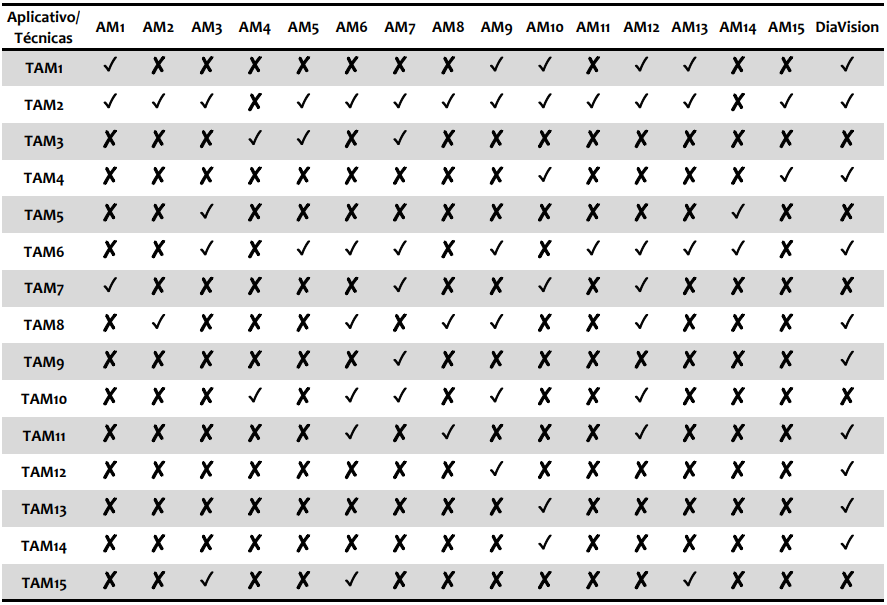
\includegraphics[scale=0.68]{Imagens/proposta/tecnicas_propostas.png}
      \end{center}
      \legend{Fonte: Autor.}
\end{table}

\section{Considerações Finais}

Este capítulo buscou realizar um levantamento, por meio de um estudo de MSL, do estado da arte
acerca dos problemas de acessibilidade enfrentados por PDV e das soluções para os mesmos.
A partir da análise dos resultados, ficou evidente a necessidade de preocupação com
acessibilidade no processo desenvolvimento de soluções para dispositivos móveis.
Sendo identificadas 15 das principais soluções para resolver diferentes problemas relacionados à DV,
das quais 10 foram consideradas no desenvolvimento da solução proposta,
que será descrita no próximo capítulo.